\documentclass[msc]{mestrado}

%%\usepackage{fullpage, epic, eepic}
\usepackage{master}

%% Inicio do documento
\begin{document}
\mainmatter

\headsep=40pt
\oddsidemargin=15pt
\begin{spacing}{1.4}
\parskip=6pt


\begin{figure}%
%\begin{sidewaysfigure}
  \centering
  \subfloat[\textbf{Linux$^{\mathbf{Std}}$ - Interrup��o} \newline \vskip
  1mm VM: 8.6, DP: 1.5, Min: 8.8, Max: 15.6 ]{%
    \label{fig:ker23Sem}%
    {\scalebox{0.58}{% GNUPLOT: LaTeX picture with Postscript
\begingroup
  \makeatletter
  \providecommand\color[2][]{%
    \GenericError{(gnuplot) \space\space\space\@spaces}{%
      Package color not loaded in conjunction with
      terminal option `colourtext'%
    }{See the gnuplot documentation for explanation.%
    }{Either use 'blacktext' in gnuplot or load the package
      color.sty in LaTeX.}%
    \renewcommand\color[2][]{}%
  }%
  \providecommand\includegraphics[2][]{%
    \GenericError{(gnuplot) \space\space\space\@spaces}{%
      Package graphicx or graphics not loaded%
    }{See the gnuplot documentation for explanation.%
    }{The gnuplot epslatex terminal needs graphicx.sty or graphics.sty.}%
    \renewcommand\includegraphics[2][]{}%
  }%
  \providecommand\rotatebox[2]{#2}%
  \@ifundefined{ifGPcolor}{%
    \newif\ifGPcolor
    \GPcolorfalse
  }{}%
  \@ifundefined{ifGPblacktext}{%
    \newif\ifGPblacktext
    \GPblacktextfalse
  }{}%
  % define a \g@addto@macro without @ in the name:
  \let\gplgaddtomacro\g@addto@macro
  % define empty templates for all commands taking text:
  \gdef\gplbacktext{}%
  \gdef\gplfronttext{}%
  \makeatother
  \ifGPblacktext
    % no textcolor at all
    \def\colorrgb#1{}%
    \def\colorgray#1{}%
  \else
    % gray or color?
    \ifGPcolor
      \def\colorrgb#1{\color[rgb]{#1}}%
      \def\colorgray#1{\color[gray]{#1}}%
      \expandafter\def\csname LTw\endcsname{\color{white}}%
      \expandafter\def\csname LTb\endcsname{\color{black}}%
      \expandafter\def\csname LTa\endcsname{\color{black}}%
      \expandafter\def\csname LT0\endcsname{\color[rgb]{1,0,0}}%
      \expandafter\def\csname LT1\endcsname{\color[rgb]{0,1,0}}%
      \expandafter\def\csname LT2\endcsname{\color[rgb]{0,0,1}}%
      \expandafter\def\csname LT3\endcsname{\color[rgb]{1,0,1}}%
      \expandafter\def\csname LT4\endcsname{\color[rgb]{0,1,1}}%
      \expandafter\def\csname LT5\endcsname{\color[rgb]{1,1,0}}%
      \expandafter\def\csname LT6\endcsname{\color[rgb]{0,0,0}}%
      \expandafter\def\csname LT7\endcsname{\color[rgb]{1,0.3,0}}%
      \expandafter\def\csname LT8\endcsname{\color[rgb]{0.5,0.5,0.5}}%
    \else
      % gray
      \def\colorrgb#1{\color{black}}%
      \def\colorgray#1{\color[gray]{#1}}%
      \expandafter\def\csname LTw\endcsname{\color{white}}%
      \expandafter\def\csname LTb\endcsname{\color{black}}%
      \expandafter\def\csname LTa\endcsname{\color{black}}%
      \expandafter\def\csname LT0\endcsname{\color{black}}%
      \expandafter\def\csname LT1\endcsname{\color{black}}%
      \expandafter\def\csname LT2\endcsname{\color{black}}%
      \expandafter\def\csname LT3\endcsname{\color{black}}%
      \expandafter\def\csname LT4\endcsname{\color{black}}%
      \expandafter\def\csname LT5\endcsname{\color{black}}%
      \expandafter\def\csname LT6\endcsname{\color{black}}%
      \expandafter\def\csname LT7\endcsname{\color{black}}%
      \expandafter\def\csname LT8\endcsname{\color{black}}%
    \fi
  \fi
  \setlength{\unitlength}{0.0500bp}%
  \begin{picture}(7200.00,5040.00)%
    \gplgaddtomacro\gplbacktext{%
      \csname LTb\endcsname%
      \put(1034,594){\makebox(0,0)[r]{\strut{}$0.0$}}%
      \put(1034,1430){\makebox(0,0)[r]{\strut{}$10.0$}}%
      \put(1034,2267){\makebox(0,0)[r]{\strut{}$20.0$}}%
      \put(1034,3103){\makebox(0,0)[r]{\strut{}$30.0$}}%
      \put(1034,3940){\makebox(0,0)[r]{\strut{}$40.0$}}%
      \put(1034,4776){\makebox(0,0)[r]{\strut{}$50.0$}}%
      \put(1166,374){\makebox(0,0){\strut{}$ 0$}}%
      \put(2109,374){\makebox(0,0){\strut{}$ 10$}}%
      \put(3053,374){\makebox(0,0){\strut{}$ 20$}}%
      \put(3996,374){\makebox(0,0){\strut{}$ 30$}}%
      \put(4939,374){\makebox(0,0){\strut{}$ 40$}}%
      \put(5883,374){\makebox(0,0){\strut{}$ 50$}}%
      \put(6826,374){\makebox(0,0){\strut{}$ 60$}}%
      \put(396,2685){\rotatebox{90}{\makebox(0,0){\strut{}Latency ($\mu s$)}}}%
      \put(3996,110){\makebox(0,0){\strut{}Time ($s$)}}%
    }%
    \gplgaddtomacro\gplfronttext{%
    }%
    \gplbacktext
    \put(0,0){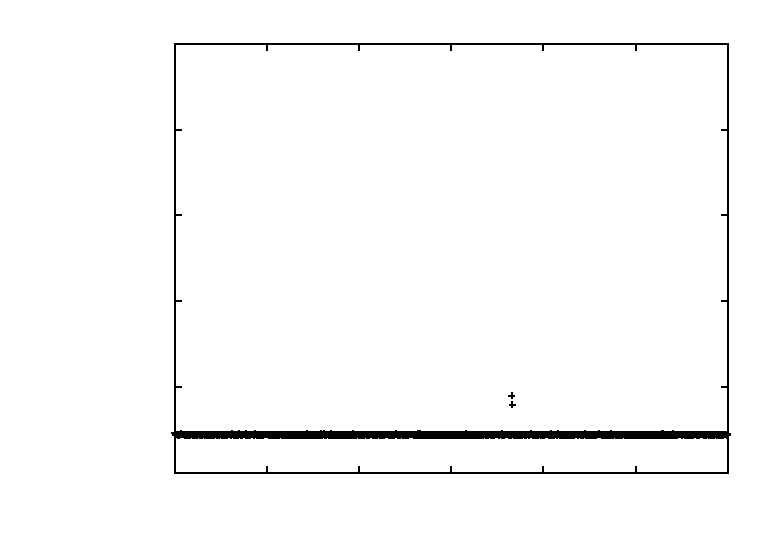
\includegraphics{fig2/ker23Sem}}%
    \gplfronttext
  \end{picture}%
\endgroup
}}} \hspace{4pt}%
  \subfloat[\textbf{Linux$^{\mathbf{Std}}$ - Ativa��o} \newline \vskip
  1mm VM: 13.4, DP: 2.6, Min: 13.2, Max: 24.4]{%
    \label{fig:ker23SemSched}%
    {\scalebox{0.58}{% GNUPLOT: LaTeX picture with Postscript
\begingroup
  \makeatletter
  \providecommand\color[2][]{%
    \GenericError{(gnuplot) \space\space\space\@spaces}{%
      Package color not loaded in conjunction with
      terminal option `colourtext'%
    }{See the gnuplot documentation for explanation.%
    }{Either use 'blacktext' in gnuplot or load the package
      color.sty in LaTeX.}%
    \renewcommand\color[2][]{}%
  }%
  \providecommand\includegraphics[2][]{%
    \GenericError{(gnuplot) \space\space\space\@spaces}{%
      Package graphicx or graphics not loaded%
    }{See the gnuplot documentation for explanation.%
    }{The gnuplot epslatex terminal needs graphicx.sty or graphics.sty.}%
    \renewcommand\includegraphics[2][]{}%
  }%
  \providecommand\rotatebox[2]{#2}%
  \@ifundefined{ifGPcolor}{%
    \newif\ifGPcolor
    \GPcolorfalse
  }{}%
  \@ifundefined{ifGPblacktext}{%
    \newif\ifGPblacktext
    \GPblacktextfalse
  }{}%
  % define a \g@addto@macro without @ in the name:
  \let\gplgaddtomacro\g@addto@macro
  % define empty templates for all commands taking text:
  \gdef\gplbacktext{}%
  \gdef\gplfronttext{}%
  \makeatother
  \ifGPblacktext
    % no textcolor at all
    \def\colorrgb#1{}%
    \def\colorgray#1{}%
  \else
    % gray or color?
    \ifGPcolor
      \def\colorrgb#1{\color[rgb]{#1}}%
      \def\colorgray#1{\color[gray]{#1}}%
      \expandafter\def\csname LTw\endcsname{\color{white}}%
      \expandafter\def\csname LTb\endcsname{\color{black}}%
      \expandafter\def\csname LTa\endcsname{\color{black}}%
      \expandafter\def\csname LT0\endcsname{\color[rgb]{1,0,0}}%
      \expandafter\def\csname LT1\endcsname{\color[rgb]{0,1,0}}%
      \expandafter\def\csname LT2\endcsname{\color[rgb]{0,0,1}}%
      \expandafter\def\csname LT3\endcsname{\color[rgb]{1,0,1}}%
      \expandafter\def\csname LT4\endcsname{\color[rgb]{0,1,1}}%
      \expandafter\def\csname LT5\endcsname{\color[rgb]{1,1,0}}%
      \expandafter\def\csname LT6\endcsname{\color[rgb]{0,0,0}}%
      \expandafter\def\csname LT7\endcsname{\color[rgb]{1,0.3,0}}%
      \expandafter\def\csname LT8\endcsname{\color[rgb]{0.5,0.5,0.5}}%
    \else
      % gray
      \def\colorrgb#1{\color{black}}%
      \def\colorgray#1{\color[gray]{#1}}%
      \expandafter\def\csname LTw\endcsname{\color{white}}%
      \expandafter\def\csname LTb\endcsname{\color{black}}%
      \expandafter\def\csname LTa\endcsname{\color{black}}%
      \expandafter\def\csname LT0\endcsname{\color{black}}%
      \expandafter\def\csname LT1\endcsname{\color{black}}%
      \expandafter\def\csname LT2\endcsname{\color{black}}%
      \expandafter\def\csname LT3\endcsname{\color{black}}%
      \expandafter\def\csname LT4\endcsname{\color{black}}%
      \expandafter\def\csname LT5\endcsname{\color{black}}%
      \expandafter\def\csname LT6\endcsname{\color{black}}%
      \expandafter\def\csname LT7\endcsname{\color{black}}%
      \expandafter\def\csname LT8\endcsname{\color{black}}%
    \fi
  \fi
  \setlength{\unitlength}{0.0500bp}%
  \begin{picture}(7200.00,5040.00)%
    \gplgaddtomacro\gplbacktext{%
      \csname LTb\endcsname%
      \put(1034,594){\makebox(0,0)[r]{\strut{}$0.0$}}%
      \put(1034,1640){\makebox(0,0)[r]{\strut{}$5.0$}}%
      \put(1034,2685){\makebox(0,0)[r]{\strut{}$10.0$}}%
      \put(1034,3731){\makebox(0,0)[r]{\strut{}$15.0$}}%
      \put(1034,4776){\makebox(0,0)[r]{\strut{}$20.0$}}%
      \put(1166,374){\makebox(0,0){\strut{}$ 0$}}%
      \put(2109,374){\makebox(0,0){\strut{}$ 10$}}%
      \put(3053,374){\makebox(0,0){\strut{}$ 20$}}%
      \put(3996,374){\makebox(0,0){\strut{}$ 30$}}%
      \put(4939,374){\makebox(0,0){\strut{}$ 40$}}%
      \put(5883,374){\makebox(0,0){\strut{}$ 50$}}%
      \put(6826,374){\makebox(0,0){\strut{}$ 60$}}%
      \put(396,2685){\rotatebox{90}{\makebox(0,0){\strut{}Lat\^encia em $\mu s$}}}%
      \put(3996,110){\makebox(0,0){\strut{}Tempo de observa\c{c}\~ao em $s$}}%
    }%
    \gplgaddtomacro\gplfronttext{%
    }%
    \gplbacktext
    \put(0,0){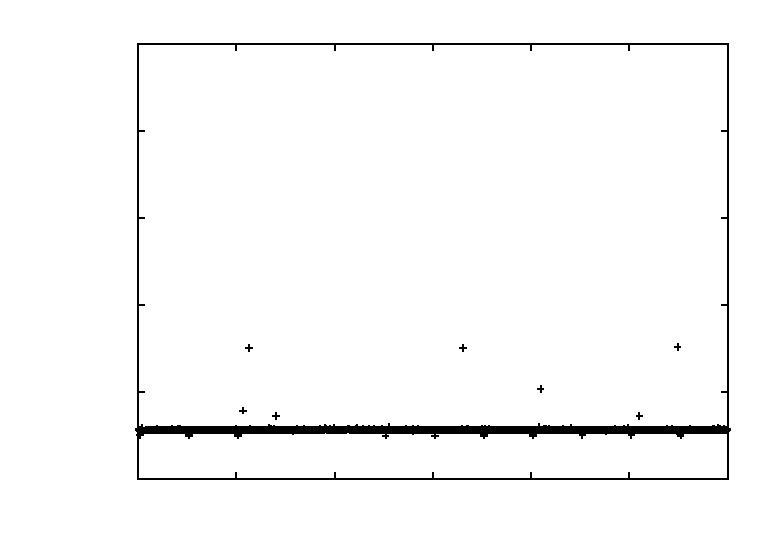
\includegraphics{fig/ker23SemSched}}%
    \gplfronttext
  \end{picture}%
\endgroup
}}}


  \subfloat[\textbf{Linux$^{\mathbf{Std}}$ - Interrup��o} \newline \vskip 1mm VM:
  10.3, DP: 2.9, Min: 9.2, Max: 52.4]{%
    \label{fig:ker23Tot}%
    {\scalebox{0.58}{% GNUPLOT: LaTeX picture with Postscript
\begingroup
  \makeatletter
  \providecommand\color[2][]{%
    \GenericError{(gnuplot) \space\space\space\@spaces}{%
      Package color not loaded in conjunction with
      terminal option `colourtext'%
    }{See the gnuplot documentation for explanation.%
    }{Either use 'blacktext' in gnuplot or load the package
      color.sty in LaTeX.}%
    \renewcommand\color[2][]{}%
  }%
  \providecommand\includegraphics[2][]{%
    \GenericError{(gnuplot) \space\space\space\@spaces}{%
      Package graphicx or graphics not loaded%
    }{See the gnuplot documentation for explanation.%
    }{The gnuplot epslatex terminal needs graphicx.sty or graphics.sty.}%
    \renewcommand\includegraphics[2][]{}%
  }%
  \providecommand\rotatebox[2]{#2}%
  \@ifundefined{ifGPcolor}{%
    \newif\ifGPcolor
    \GPcolorfalse
  }{}%
  \@ifundefined{ifGPblacktext}{%
    \newif\ifGPblacktext
    \GPblacktextfalse
  }{}%
  % define a \g@addto@macro without @ in the name:
  \let\gplgaddtomacro\g@addto@macro
  % define empty templates for all commands taking text:
  \gdef\gplbacktext{}%
  \gdef\gplfronttext{}%
  \makeatother
  \ifGPblacktext
    % no textcolor at all
    \def\colorrgb#1{}%
    \def\colorgray#1{}%
  \else
    % gray or color?
    \ifGPcolor
      \def\colorrgb#1{\color[rgb]{#1}}%
      \def\colorgray#1{\color[gray]{#1}}%
      \expandafter\def\csname LTw\endcsname{\color{white}}%
      \expandafter\def\csname LTb\endcsname{\color{black}}%
      \expandafter\def\csname LTa\endcsname{\color{black}}%
      \expandafter\def\csname LT0\endcsname{\color[rgb]{1,0,0}}%
      \expandafter\def\csname LT1\endcsname{\color[rgb]{0,1,0}}%
      \expandafter\def\csname LT2\endcsname{\color[rgb]{0,0,1}}%
      \expandafter\def\csname LT3\endcsname{\color[rgb]{1,0,1}}%
      \expandafter\def\csname LT4\endcsname{\color[rgb]{0,1,1}}%
      \expandafter\def\csname LT5\endcsname{\color[rgb]{1,1,0}}%
      \expandafter\def\csname LT6\endcsname{\color[rgb]{0,0,0}}%
      \expandafter\def\csname LT7\endcsname{\color[rgb]{1,0.3,0}}%
      \expandafter\def\csname LT8\endcsname{\color[rgb]{0.5,0.5,0.5}}%
    \else
      % gray
      \def\colorrgb#1{\color{black}}%
      \def\colorgray#1{\color[gray]{#1}}%
      \expandafter\def\csname LTw\endcsname{\color{white}}%
      \expandafter\def\csname LTb\endcsname{\color{black}}%
      \expandafter\def\csname LTa\endcsname{\color{black}}%
      \expandafter\def\csname LT0\endcsname{\color{black}}%
      \expandafter\def\csname LT1\endcsname{\color{black}}%
      \expandafter\def\csname LT2\endcsname{\color{black}}%
      \expandafter\def\csname LT3\endcsname{\color{black}}%
      \expandafter\def\csname LT4\endcsname{\color{black}}%
      \expandafter\def\csname LT5\endcsname{\color{black}}%
      \expandafter\def\csname LT6\endcsname{\color{black}}%
      \expandafter\def\csname LT7\endcsname{\color{black}}%
      \expandafter\def\csname LT8\endcsname{\color{black}}%
    \fi
  \fi
  \setlength{\unitlength}{0.0500bp}%
  \begin{picture}(7200.00,5040.00)%
    \gplgaddtomacro\gplbacktext{%
      \csname LTb\endcsname%
      \put(1034,594){\makebox(0,0)[r]{\strut{}$0.0$}}%
      \put(1034,1430){\makebox(0,0)[r]{\strut{}$10.0$}}%
      \put(1034,2267){\makebox(0,0)[r]{\strut{}$20.0$}}%
      \put(1034,3103){\makebox(0,0)[r]{\strut{}$30.0$}}%
      \put(1034,3940){\makebox(0,0)[r]{\strut{}$40.0$}}%
      \put(1034,4776){\makebox(0,0)[r]{\strut{}$50.0$}}%
      \put(1166,374){\makebox(0,0){\strut{}$ 0$}}%
      \put(2109,374){\makebox(0,0){\strut{}$ 10$}}%
      \put(3053,374){\makebox(0,0){\strut{}$ 20$}}%
      \put(3996,374){\makebox(0,0){\strut{}$ 30$}}%
      \put(4939,374){\makebox(0,0){\strut{}$ 40$}}%
      \put(5883,374){\makebox(0,0){\strut{}$ 50$}}%
      \put(6826,374){\makebox(0,0){\strut{}$ 60$}}%
      \put(396,2685){\rotatebox{90}{\makebox(0,0){\strut{}Latency ($\mu s$)}}}%
      \put(3996,110){\makebox(0,0){\strut{}Time ($s$)}}%
    }%
    \gplgaddtomacro\gplfronttext{%
    }%
    \gplbacktext
    \put(0,0){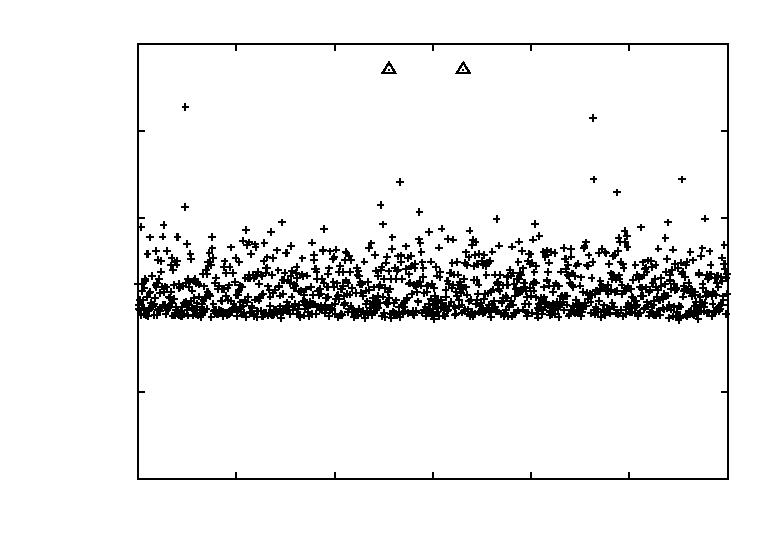
\includegraphics{fig/ker23Tot}}%
    \gplfronttext
  \end{picture}%
\endgroup
}}} \hspace{4pt}%
  \subfloat[\textbf{Linux$^{\mathbf{Std}}$ - Ativa��o}\newline\vskip 1mm VM: 287.1,
  DP: 783.3, Min: 45.1, Max: 14281.3]{%
    \label{fig:ker23TotSched}%
    {\scalebox{0.58}{% GNUPLOT: LaTeX picture with Postscript
\begingroup
  \makeatletter
  \providecommand\color[2][]{%
    \GenericError{(gnuplot) \space\space\space\@spaces}{%
      Package color not loaded in conjunction with
      terminal option `colourtext'%
    }{See the gnuplot documentation for explanation.%
    }{Either use 'blacktext' in gnuplot or load the package
      color.sty in LaTeX.}%
    \renewcommand\color[2][]{}%
  }%
  \providecommand\includegraphics[2][]{%
    \GenericError{(gnuplot) \space\space\space\@spaces}{%
      Package graphicx or graphics not loaded%
    }{See the gnuplot documentation for explanation.%
    }{The gnuplot epslatex terminal needs graphicx.sty or graphics.sty.}%
    \renewcommand\includegraphics[2][]{}%
  }%
  \providecommand\rotatebox[2]{#2}%
  \@ifundefined{ifGPcolor}{%
    \newif\ifGPcolor
    \GPcolorfalse
  }{}%
  \@ifundefined{ifGPblacktext}{%
    \newif\ifGPblacktext
    \GPblacktextfalse
  }{}%
  % define a \g@addto@macro without @ in the name:
  \let\gplgaddtomacro\g@addto@macro
  % define empty templates for all commands taking text:
  \gdef\gplbacktext{}%
  \gdef\gplfronttext{}%
  \makeatother
  \ifGPblacktext
    % no textcolor at all
    \def\colorrgb#1{}%
    \def\colorgray#1{}%
  \else
    % gray or color?
    \ifGPcolor
      \def\colorrgb#1{\color[rgb]{#1}}%
      \def\colorgray#1{\color[gray]{#1}}%
      \expandafter\def\csname LTw\endcsname{\color{white}}%
      \expandafter\def\csname LTb\endcsname{\color{black}}%
      \expandafter\def\csname LTa\endcsname{\color{black}}%
      \expandafter\def\csname LT0\endcsname{\color[rgb]{1,0,0}}%
      \expandafter\def\csname LT1\endcsname{\color[rgb]{0,1,0}}%
      \expandafter\def\csname LT2\endcsname{\color[rgb]{0,0,1}}%
      \expandafter\def\csname LT3\endcsname{\color[rgb]{1,0,1}}%
      \expandafter\def\csname LT4\endcsname{\color[rgb]{0,1,1}}%
      \expandafter\def\csname LT5\endcsname{\color[rgb]{1,1,0}}%
      \expandafter\def\csname LT6\endcsname{\color[rgb]{0,0,0}}%
      \expandafter\def\csname LT7\endcsname{\color[rgb]{1,0.3,0}}%
      \expandafter\def\csname LT8\endcsname{\color[rgb]{0.5,0.5,0.5}}%
    \else
      % gray
      \def\colorrgb#1{\color{black}}%
      \def\colorgray#1{\color[gray]{#1}}%
      \expandafter\def\csname LTw\endcsname{\color{white}}%
      \expandafter\def\csname LTb\endcsname{\color{black}}%
      \expandafter\def\csname LTa\endcsname{\color{black}}%
      \expandafter\def\csname LT0\endcsname{\color{black}}%
      \expandafter\def\csname LT1\endcsname{\color{black}}%
      \expandafter\def\csname LT2\endcsname{\color{black}}%
      \expandafter\def\csname LT3\endcsname{\color{black}}%
      \expandafter\def\csname LT4\endcsname{\color{black}}%
      \expandafter\def\csname LT5\endcsname{\color{black}}%
      \expandafter\def\csname LT6\endcsname{\color{black}}%
      \expandafter\def\csname LT7\endcsname{\color{black}}%
      \expandafter\def\csname LT8\endcsname{\color{black}}%
    \fi
  \fi
  \setlength{\unitlength}{0.0500bp}%
  \begin{picture}(7200.00,5040.00)%
    \gplgaddtomacro\gplbacktext{%
      \csname LTb\endcsname%
      \put(1034,594){\makebox(0,0)[r]{\strut{}$0.0$}}%
      \put(1034,1430){\makebox(0,0)[r]{\strut{}$10.0$}}%
      \put(1034,2267){\makebox(0,0)[r]{\strut{}$20.0$}}%
      \put(1034,3103){\makebox(0,0)[r]{\strut{}$30.0$}}%
      \put(1034,3940){\makebox(0,0)[r]{\strut{}$40.0$}}%
      \put(1034,4776){\makebox(0,0)[r]{\strut{}$50.0$}}%
      \put(1166,374){\makebox(0,0){\strut{}$ 0$}}%
      \put(2109,374){\makebox(0,0){\strut{}$ 10$}}%
      \put(3053,374){\makebox(0,0){\strut{}$ 20$}}%
      \put(3996,374){\makebox(0,0){\strut{}$ 30$}}%
      \put(4939,374){\makebox(0,0){\strut{}$ 40$}}%
      \put(5883,374){\makebox(0,0){\strut{}$ 50$}}%
      \put(6826,374){\makebox(0,0){\strut{}$ 60$}}%
      \put(396,2685){\rotatebox{90}{\makebox(0,0){\strut{}Latency ($\mu s$)}}}%
      \put(3996,110){\makebox(0,0){\strut{}Time ($s$)}}%
    }%
    \gplgaddtomacro\gplfronttext{%
    }%
    \gplbacktext
    \put(0,0){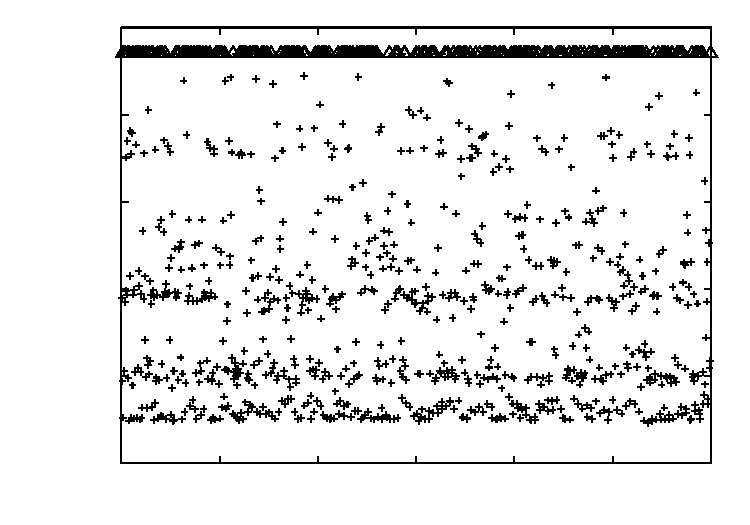
\includegraphics{fig2/ker23TotSched}}%
    \gplfronttext
  \end{picture}%
\endgroup
}}}

  \caption[]{Lat�ncia
    de interrup��o e de ativa��o do \kernell Linux, vers�o 2.6.23.9, op��o
    \ing{Low-Latency}. As figuras \subref{fig:ker23Sem} e \subref{fig:ker23SemSched}
    representam uma execu��o sem estresse. As figuras \subref{fig:ker23Udp} e
    \subref{fig:ker23UdpSched} representam uma execu��o com estresse de comunica��o
    UDP.  As figuras \subref{fig:ker23Tot} e \subref{fig:ker23TotSched} representam
    uma execu��o com estresse de comunica��o UDP e uma carga extra do processador. A
    freq��ncia de escrita na porta paralela � de $20 Hz$.}
  \label{fig:ker2619}%
\end{figure}


\end{spacing}

%% Fim do documento
\end{document}

\begin{figure}[!hbt]
  %\hfill
  %\vspace{0.2in}
  \begin{minipage}[!t]{\textwidth}
    \begin{center}  
      \centerline{\resizebox{0.5\linewidth}{!}{% GNUPLOT: LaTeX picture with Postscript
\begingroup
  \makeatletter
  \providecommand\color[2][]{%
    \GenericError{(gnuplot) \space\space\space\@spaces}{%
      Package color not loaded in conjunction with
      terminal option `colourtext'%
    }{See the gnuplot documentation for explanation.%
    }{Either use 'blacktext' in gnuplot or load the package
      color.sty in LaTeX.}%
    \renewcommand\color[2][]{}%
  }%
  \providecommand\includegraphics[2][]{%
    \GenericError{(gnuplot) \space\space\space\@spaces}{%
      Package graphicx or graphics not loaded%
    }{See the gnuplot documentation for explanation.%
    }{The gnuplot epslatex terminal needs graphicx.sty or graphics.sty.}%
    \renewcommand\includegraphics[2][]{}%
  }%
  \providecommand\rotatebox[2]{#2}%
  \@ifundefined{ifGPcolor}{%
    \newif\ifGPcolor
    \GPcolorfalse
  }{}%
  \@ifundefined{ifGPblacktext}{%
    \newif\ifGPblacktext
    \GPblacktextfalse
  }{}%
  % define a \g@addto@macro without @ in the name:
  \let\gplgaddtomacro\g@addto@macro
  % define empty templates for all commands taking text:
  \gdef\gplbacktext{}%
  \gdef\gplfronttext{}%
  \makeatother
  \ifGPblacktext
    % no textcolor at all
    \def\colorrgb#1{}%
    \def\colorgray#1{}%
  \else
    % gray or color?
    \ifGPcolor
      \def\colorrgb#1{\color[rgb]{#1}}%
      \def\colorgray#1{\color[gray]{#1}}%
      \expandafter\def\csname LTw\endcsname{\color{white}}%
      \expandafter\def\csname LTb\endcsname{\color{black}}%
      \expandafter\def\csname LTa\endcsname{\color{black}}%
      \expandafter\def\csname LT0\endcsname{\color[rgb]{1,0,0}}%
      \expandafter\def\csname LT1\endcsname{\color[rgb]{0,1,0}}%
      \expandafter\def\csname LT2\endcsname{\color[rgb]{0,0,1}}%
      \expandafter\def\csname LT3\endcsname{\color[rgb]{1,0,1}}%
      \expandafter\def\csname LT4\endcsname{\color[rgb]{0,1,1}}%
      \expandafter\def\csname LT5\endcsname{\color[rgb]{1,1,0}}%
      \expandafter\def\csname LT6\endcsname{\color[rgb]{0,0,0}}%
      \expandafter\def\csname LT7\endcsname{\color[rgb]{1,0.3,0}}%
      \expandafter\def\csname LT8\endcsname{\color[rgb]{0.5,0.5,0.5}}%
    \else
      % gray
      \def\colorrgb#1{\color{black}}%
      \def\colorgray#1{\color[gray]{#1}}%
      \expandafter\def\csname LTw\endcsname{\color{white}}%
      \expandafter\def\csname LTb\endcsname{\color{black}}%
      \expandafter\def\csname LTa\endcsname{\color{black}}%
      \expandafter\def\csname LT0\endcsname{\color{black}}%
      \expandafter\def\csname LT1\endcsname{\color{black}}%
      \expandafter\def\csname LT2\endcsname{\color{black}}%
      \expandafter\def\csname LT3\endcsname{\color{black}}%
      \expandafter\def\csname LT4\endcsname{\color{black}}%
      \expandafter\def\csname LT5\endcsname{\color{black}}%
      \expandafter\def\csname LT6\endcsname{\color{black}}%
      \expandafter\def\csname LT7\endcsname{\color{black}}%
      \expandafter\def\csname LT8\endcsname{\color{black}}%
    \fi
  \fi
  \setlength{\unitlength}{0.0500bp}%
  \begin{picture}(7200.00,5040.00)%
    \gplgaddtomacro\gplbacktext{%
      \csname LTb\endcsname%
      \put(1518,660){\makebox(0,0)[r]{\strut{}$0.0$}}%
      \put(1518,1175){\makebox(0,0)[r]{\strut{}$1000.0$}}%
      \put(1518,1689){\makebox(0,0)[r]{\strut{}$2000.0$}}%
      \put(1518,2204){\makebox(0,0)[r]{\strut{}$3000.0$}}%
      \put(1518,2718){\makebox(0,0)[r]{\strut{}$4000.0$}}%
      \put(1518,3233){\makebox(0,0)[r]{\strut{}$5000.0$}}%
      \put(1518,3747){\makebox(0,0)[r]{\strut{}$6000.0$}}%
      \put(1518,4262){\makebox(0,0)[r]{\strut{}$7000.0$}}%
      \put(1518,4776){\makebox(0,0)[r]{\strut{}$8000.0$}}%
      \put(1650,440){\makebox(0,0){\strut{}$ 0$}}%
      \put(2389,440){\makebox(0,0){\strut{}$ 10$}}%
      \put(3129,440){\makebox(0,0){\strut{}$ 20$}}%
      \put(3868,440){\makebox(0,0){\strut{}$ 30$}}%
      \put(4608,440){\makebox(0,0){\strut{}$ 40$}}%
      \put(5347,440){\makebox(0,0){\strut{}$ 50$}}%
      \put(6087,440){\makebox(0,0){\strut{}$ 60$}}%
      \put(6826,440){\makebox(0,0){\strut{}$ 70$}}%
      \put(220,2718){\rotatebox{90}{\makebox(0,0){\strut{}Lat\^encia em $\mu s$}}}%
      \put(4238,110){\makebox(0,0){\strut{}Tempo de execu\c{c}\~ao em $s$}}%
    }%
    \gplgaddtomacro\gplfronttext{%
    }%
    \gplbacktext
    \put(0,0){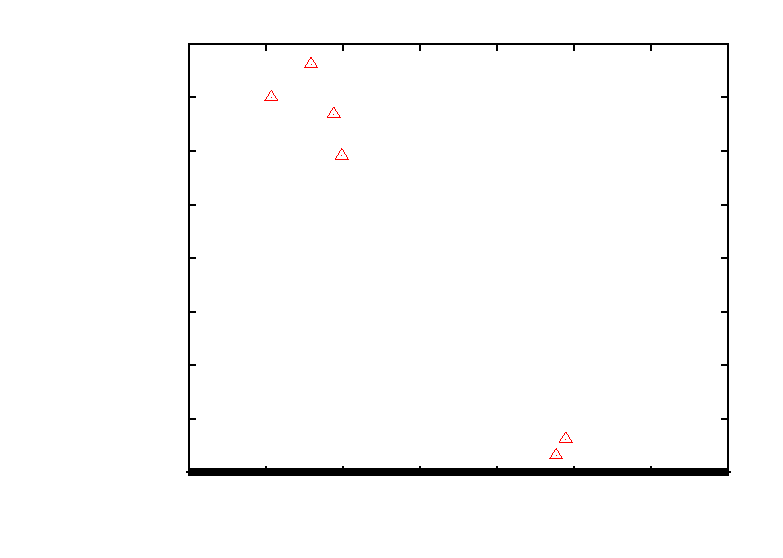
\includegraphics{fig/klight1}}%
    \gplfronttext
  \end{picture}%
\endgroup
}}
      \caption{Lat�ncia de interrup��o do \kernell Linux}
      \label{fig:irqKern}
    \end{center}
  \end{minipage}
  %\hfill
  \\
  \vspace{.4in}
  \begin{minipage}[!t]{\textwidth}
    \begin{center}  
      \centerline{\resizebox{0.5\linewidth}{!}{% GNUPLOT: LaTeX picture with Postscript
\begingroup
  \makeatletter
  \providecommand\color[2][]{%
    \GenericError{(gnuplot) \space\space\space\@spaces}{%
      Package color not loaded in conjunction with
      terminal option `colourtext'%
    }{See the gnuplot documentation for explanation.%
    }{Either use 'blacktext' in gnuplot or load the package
      color.sty in LaTeX.}%
    \renewcommand\color[2][]{}%
  }%
  \providecommand\includegraphics[2][]{%
    \GenericError{(gnuplot) \space\space\space\@spaces}{%
      Package graphicx or graphics not loaded%
    }{See the gnuplot documentation for explanation.%
    }{The gnuplot epslatex terminal needs graphicx.sty or graphics.sty.}%
    \renewcommand\includegraphics[2][]{}%
  }%
  \providecommand\rotatebox[2]{#2}%
  \@ifundefined{ifGPcolor}{%
    \newif\ifGPcolor
    \GPcolorfalse
  }{}%
  \@ifundefined{ifGPblacktext}{%
    \newif\ifGPblacktext
    \GPblacktextfalse
  }{}%
  % define a \g@addto@macro without @ in the name:
  \let\gplgaddtomacro\g@addto@macro
  % define empty templates for all commands taking text:
  \gdef\gplbacktext{}%
  \gdef\gplfronttext{}%
  \makeatother
  \ifGPblacktext
    % no textcolor at all
    \def\colorrgb#1{}%
    \def\colorgray#1{}%
  \else
    % gray or color?
    \ifGPcolor
      \def\colorrgb#1{\color[rgb]{#1}}%
      \def\colorgray#1{\color[gray]{#1}}%
      \expandafter\def\csname LTw\endcsname{\color{white}}%
      \expandafter\def\csname LTb\endcsname{\color{black}}%
      \expandafter\def\csname LTa\endcsname{\color{black}}%
      \expandafter\def\csname LT0\endcsname{\color[rgb]{1,0,0}}%
      \expandafter\def\csname LT1\endcsname{\color[rgb]{0,1,0}}%
      \expandafter\def\csname LT2\endcsname{\color[rgb]{0,0,1}}%
      \expandafter\def\csname LT3\endcsname{\color[rgb]{1,0,1}}%
      \expandafter\def\csname LT4\endcsname{\color[rgb]{0,1,1}}%
      \expandafter\def\csname LT5\endcsname{\color[rgb]{1,1,0}}%
      \expandafter\def\csname LT6\endcsname{\color[rgb]{0,0,0}}%
      \expandafter\def\csname LT7\endcsname{\color[rgb]{1,0.3,0}}%
      \expandafter\def\csname LT8\endcsname{\color[rgb]{0.5,0.5,0.5}}%
    \else
      % gray
      \def\colorrgb#1{\color{black}}%
      \def\colorgray#1{\color[gray]{#1}}%
      \expandafter\def\csname LTw\endcsname{\color{white}}%
      \expandafter\def\csname LTb\endcsname{\color{black}}%
      \expandafter\def\csname LTa\endcsname{\color{black}}%
      \expandafter\def\csname LT0\endcsname{\color{black}}%
      \expandafter\def\csname LT1\endcsname{\color{black}}%
      \expandafter\def\csname LT2\endcsname{\color{black}}%
      \expandafter\def\csname LT3\endcsname{\color{black}}%
      \expandafter\def\csname LT4\endcsname{\color{black}}%
      \expandafter\def\csname LT5\endcsname{\color{black}}%
      \expandafter\def\csname LT6\endcsname{\color{black}}%
      \expandafter\def\csname LT7\endcsname{\color{black}}%
      \expandafter\def\csname LT8\endcsname{\color{black}}%
    \fi
  \fi
  \setlength{\unitlength}{0.0500bp}%
  \begin{picture}(7200.00,5040.00)%
    \gplgaddtomacro\gplbacktext{%
      \csname LTb\endcsname%
      \put(1254,660){\makebox(0,0)[r]{\strut{}$8.0$}}%
      \put(1254,1175){\makebox(0,0)[r]{\strut{}$9.0$}}%
      \put(1254,1689){\makebox(0,0)[r]{\strut{}$10.0$}}%
      \put(1254,2204){\makebox(0,0)[r]{\strut{}$11.0$}}%
      \put(1254,2718){\makebox(0,0)[r]{\strut{}$12.0$}}%
      \put(1254,3233){\makebox(0,0)[r]{\strut{}$13.0$}}%
      \put(1254,3747){\makebox(0,0)[r]{\strut{}$14.0$}}%
      \put(1254,4262){\makebox(0,0)[r]{\strut{}$15.0$}}%
      \put(1254,4776){\makebox(0,0)[r]{\strut{}$16.0$}}%
      \put(1386,440){\makebox(0,0){\strut{}$ 0$}}%
      \put(2163,440){\makebox(0,0){\strut{}$ 10$}}%
      \put(2940,440){\makebox(0,0){\strut{}$ 20$}}%
      \put(3717,440){\makebox(0,0){\strut{}$ 30$}}%
      \put(4495,440){\makebox(0,0){\strut{}$ 40$}}%
      \put(5272,440){\makebox(0,0){\strut{}$ 50$}}%
      \put(6049,440){\makebox(0,0){\strut{}$ 60$}}%
      \put(6826,440){\makebox(0,0){\strut{}$ 70$}}%
      \put(220,2718){\rotatebox{90}{\makebox(0,0){\strut{}Lat\^encia em $\mu s$}}}%
      \put(4106,110){\makebox(0,0){\strut{}Tempo de execu\c{c}\~ao em $s$}}%
    }%
    \gplgaddtomacro\gplfronttext{%
    }%
    \gplbacktext
    \put(0,0){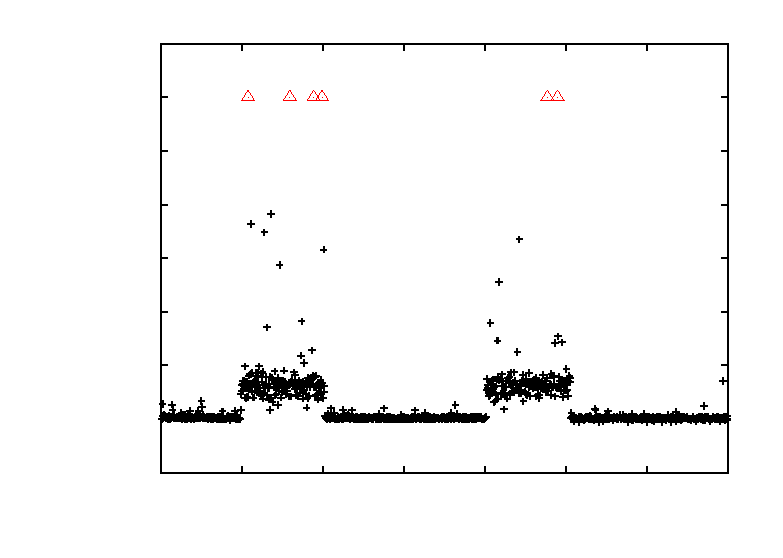
\includegraphics{fig/klight2}}%
    \gplfronttext
  \end{picture}%
\endgroup
}}
      \caption{Lat�ncia de interrup��o do \kernell Linux (m�dia sobre 10 valores)}
      \label{fig:irqKernMean}
    \end{center}
  \end{minipage}
  %\hfill
  \\
  \vspace{.4in}
  \begin{minipage}[!t]{\textwidth}
    \begin{center}  
      \centerline{\resizebox{0.5\linewidth}{!}{% GNUPLOT: LaTeX picture with Postscript
\begingroup
  \makeatletter
  \providecommand\color[2][]{%
    \GenericError{(gnuplot) \space\space\space\@spaces}{%
      Package color not loaded in conjunction with
      terminal option `colourtext'%
    }{See the gnuplot documentation for explanation.%
    }{Either use 'blacktext' in gnuplot or load the package
      color.sty in LaTeX.}%
    \renewcommand\color[2][]{}%
  }%
  \providecommand\includegraphics[2][]{%
    \GenericError{(gnuplot) \space\space\space\@spaces}{%
      Package graphicx or graphics not loaded%
    }{See the gnuplot documentation for explanation.%
    }{The gnuplot epslatex terminal needs graphicx.sty or graphics.sty.}%
    \renewcommand\includegraphics[2][]{}%
  }%
  \providecommand\rotatebox[2]{#2}%
  \@ifundefined{ifGPcolor}{%
    \newif\ifGPcolor
    \GPcolorfalse
  }{}%
  \@ifundefined{ifGPblacktext}{%
    \newif\ifGPblacktext
    \GPblacktextfalse
  }{}%
  % define a \g@addto@macro without @ in the name:
  \let\gplgaddtomacro\g@addto@macro
  % define empty templates for all commands taking text:
  \gdef\gplbacktext{}%
  \gdef\gplfronttext{}%
  \makeatother
  \ifGPblacktext
    % no textcolor at all
    \def\colorrgb#1{}%
    \def\colorgray#1{}%
  \else
    % gray or color?
    \ifGPcolor
      \def\colorrgb#1{\color[rgb]{#1}}%
      \def\colorgray#1{\color[gray]{#1}}%
      \expandafter\def\csname LTw\endcsname{\color{white}}%
      \expandafter\def\csname LTb\endcsname{\color{black}}%
      \expandafter\def\csname LTa\endcsname{\color{black}}%
      \expandafter\def\csname LT0\endcsname{\color[rgb]{1,0,0}}%
      \expandafter\def\csname LT1\endcsname{\color[rgb]{0,1,0}}%
      \expandafter\def\csname LT2\endcsname{\color[rgb]{0,0,1}}%
      \expandafter\def\csname LT3\endcsname{\color[rgb]{1,0,1}}%
      \expandafter\def\csname LT4\endcsname{\color[rgb]{0,1,1}}%
      \expandafter\def\csname LT5\endcsname{\color[rgb]{1,1,0}}%
      \expandafter\def\csname LT6\endcsname{\color[rgb]{0,0,0}}%
      \expandafter\def\csname LT7\endcsname{\color[rgb]{1,0.3,0}}%
      \expandafter\def\csname LT8\endcsname{\color[rgb]{0.5,0.5,0.5}}%
    \else
      % gray
      \def\colorrgb#1{\color{black}}%
      \def\colorgray#1{\color[gray]{#1}}%
      \expandafter\def\csname LTw\endcsname{\color{white}}%
      \expandafter\def\csname LTb\endcsname{\color{black}}%
      \expandafter\def\csname LTa\endcsname{\color{black}}%
      \expandafter\def\csname LT0\endcsname{\color{black}}%
      \expandafter\def\csname LT1\endcsname{\color{black}}%
      \expandafter\def\csname LT2\endcsname{\color{black}}%
      \expandafter\def\csname LT3\endcsname{\color{black}}%
      \expandafter\def\csname LT4\endcsname{\color{black}}%
      \expandafter\def\csname LT5\endcsname{\color{black}}%
      \expandafter\def\csname LT6\endcsname{\color{black}}%
      \expandafter\def\csname LT7\endcsname{\color{black}}%
      \expandafter\def\csname LT8\endcsname{\color{black}}%
    \fi
  \fi
  \setlength{\unitlength}{0.0500bp}%
  \begin{picture}(7200.00,5040.00)%
    \gplgaddtomacro\gplbacktext{%
      \csname LTb\endcsname%
      \put(1254,660){\makebox(0,0)[r]{\strut{}$8.0$}}%
      \put(1254,1175){\makebox(0,0)[r]{\strut{}$9.0$}}%
      \put(1254,1689){\makebox(0,0)[r]{\strut{}$10.0$}}%
      \put(1254,2204){\makebox(0,0)[r]{\strut{}$11.0$}}%
      \put(1254,2718){\makebox(0,0)[r]{\strut{}$12.0$}}%
      \put(1254,3233){\makebox(0,0)[r]{\strut{}$13.0$}}%
      \put(1254,3747){\makebox(0,0)[r]{\strut{}$14.0$}}%
      \put(1254,4262){\makebox(0,0)[r]{\strut{}$15.0$}}%
      \put(1254,4776){\makebox(0,0)[r]{\strut{}$16.0$}}%
      \put(1386,440){\makebox(0,0){\strut{}$ 0$}}%
      \put(2163,440){\makebox(0,0){\strut{}$ 10$}}%
      \put(2940,440){\makebox(0,0){\strut{}$ 20$}}%
      \put(3717,440){\makebox(0,0){\strut{}$ 30$}}%
      \put(4495,440){\makebox(0,0){\strut{}$ 40$}}%
      \put(5272,440){\makebox(0,0){\strut{}$ 50$}}%
      \put(6049,440){\makebox(0,0){\strut{}$ 60$}}%
      \put(6826,440){\makebox(0,0){\strut{}$ 70$}}%
      \put(220,2718){\rotatebox{90}{\makebox(0,0){\strut{}Lat\^encia em $\mu s$}}}%
      \put(4106,110){\makebox(0,0){\strut{}Tempo de execu\c{c}\~ao em $s$}}%
    }%
    \gplgaddtomacro\gplfronttext{%
    }%
    \gplbacktext
    \put(0,0){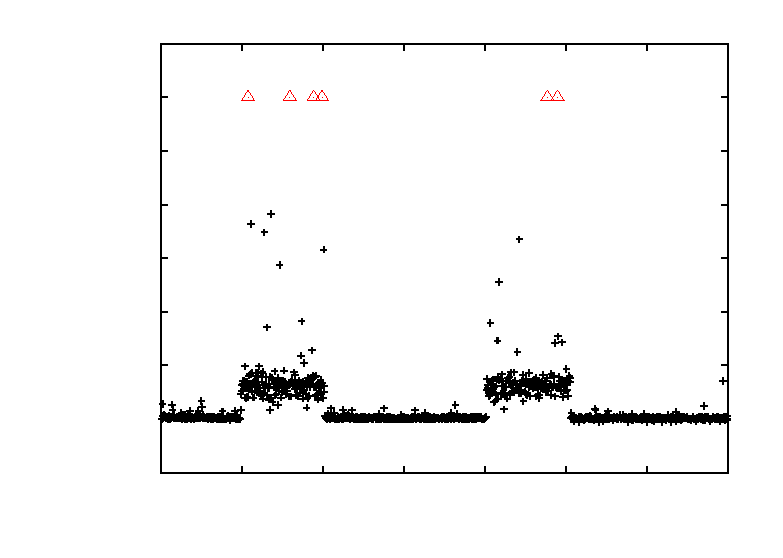
\includegraphics{fig/klight2}}%
    \gplfronttext
  \end{picture}%
\endgroup
}}
      \caption{Lat�ncia de interrup��o do \kernell Linux (m�dia sobre 10 valores)}
      \label{fig:irqKernMean}
    \end{center}
  \end{minipage}
  %\hfill
\end{figure}


% \begin{figure}
%   \begin{center}
%     % GNUPLOT: LaTeX picture with Postscript
\begingroup
  \makeatletter
  \providecommand\color[2][]{%
    \GenericError{(gnuplot) \space\space\space\@spaces}{%
      Package color not loaded in conjunction with
      terminal option `colourtext'%
    }{See the gnuplot documentation for explanation.%
    }{Either use 'blacktext' in gnuplot or load the package
      color.sty in LaTeX.}%
    \renewcommand\color[2][]{}%
  }%
  \providecommand\includegraphics[2][]{%
    \GenericError{(gnuplot) \space\space\space\@spaces}{%
      Package graphicx or graphics not loaded%
    }{See the gnuplot documentation for explanation.%
    }{The gnuplot epslatex terminal needs graphicx.sty or graphics.sty.}%
    \renewcommand\includegraphics[2][]{}%
  }%
  \providecommand\rotatebox[2]{#2}%
  \@ifundefined{ifGPcolor}{%
    \newif\ifGPcolor
    \GPcolorfalse
  }{}%
  \@ifundefined{ifGPblacktext}{%
    \newif\ifGPblacktext
    \GPblacktextfalse
  }{}%
  % define a \g@addto@macro without @ in the name:
  \let\gplgaddtomacro\g@addto@macro
  % define empty templates for all commands taking text:
  \gdef\gplbacktext{}%
  \gdef\gplfronttext{}%
  \makeatother
  \ifGPblacktext
    % no textcolor at all
    \def\colorrgb#1{}%
    \def\colorgray#1{}%
  \else
    % gray or color?
    \ifGPcolor
      \def\colorrgb#1{\color[rgb]{#1}}%
      \def\colorgray#1{\color[gray]{#1}}%
      \expandafter\def\csname LTw\endcsname{\color{white}}%
      \expandafter\def\csname LTb\endcsname{\color{black}}%
      \expandafter\def\csname LTa\endcsname{\color{black}}%
      \expandafter\def\csname LT0\endcsname{\color[rgb]{1,0,0}}%
      \expandafter\def\csname LT1\endcsname{\color[rgb]{0,1,0}}%
      \expandafter\def\csname LT2\endcsname{\color[rgb]{0,0,1}}%
      \expandafter\def\csname LT3\endcsname{\color[rgb]{1,0,1}}%
      \expandafter\def\csname LT4\endcsname{\color[rgb]{0,1,1}}%
      \expandafter\def\csname LT5\endcsname{\color[rgb]{1,1,0}}%
      \expandafter\def\csname LT6\endcsname{\color[rgb]{0,0,0}}%
      \expandafter\def\csname LT7\endcsname{\color[rgb]{1,0.3,0}}%
      \expandafter\def\csname LT8\endcsname{\color[rgb]{0.5,0.5,0.5}}%
    \else
      % gray
      \def\colorrgb#1{\color{black}}%
      \def\colorgray#1{\color[gray]{#1}}%
      \expandafter\def\csname LTw\endcsname{\color{white}}%
      \expandafter\def\csname LTb\endcsname{\color{black}}%
      \expandafter\def\csname LTa\endcsname{\color{black}}%
      \expandafter\def\csname LT0\endcsname{\color{black}}%
      \expandafter\def\csname LT1\endcsname{\color{black}}%
      \expandafter\def\csname LT2\endcsname{\color{black}}%
      \expandafter\def\csname LT3\endcsname{\color{black}}%
      \expandafter\def\csname LT4\endcsname{\color{black}}%
      \expandafter\def\csname LT5\endcsname{\color{black}}%
      \expandafter\def\csname LT6\endcsname{\color{black}}%
      \expandafter\def\csname LT7\endcsname{\color{black}}%
      \expandafter\def\csname LT8\endcsname{\color{black}}%
    \fi
  \fi
  \setlength{\unitlength}{0.0500bp}%
  \begin{picture}(7200.00,5040.00)%
    \gplgaddtomacro\gplbacktext{%
      \csname LTb\endcsname%
      \put(1518,660){\makebox(0,0)[r]{\strut{}$0.0$}}%
      \put(1518,1175){\makebox(0,0)[r]{\strut{}$1000.0$}}%
      \put(1518,1689){\makebox(0,0)[r]{\strut{}$2000.0$}}%
      \put(1518,2204){\makebox(0,0)[r]{\strut{}$3000.0$}}%
      \put(1518,2718){\makebox(0,0)[r]{\strut{}$4000.0$}}%
      \put(1518,3233){\makebox(0,0)[r]{\strut{}$5000.0$}}%
      \put(1518,3747){\makebox(0,0)[r]{\strut{}$6000.0$}}%
      \put(1518,4262){\makebox(0,0)[r]{\strut{}$7000.0$}}%
      \put(1518,4776){\makebox(0,0)[r]{\strut{}$8000.0$}}%
      \put(1650,440){\makebox(0,0){\strut{}$ 0$}}%
      \put(2389,440){\makebox(0,0){\strut{}$ 10$}}%
      \put(3129,440){\makebox(0,0){\strut{}$ 20$}}%
      \put(3868,440){\makebox(0,0){\strut{}$ 30$}}%
      \put(4608,440){\makebox(0,0){\strut{}$ 40$}}%
      \put(5347,440){\makebox(0,0){\strut{}$ 50$}}%
      \put(6087,440){\makebox(0,0){\strut{}$ 60$}}%
      \put(6826,440){\makebox(0,0){\strut{}$ 70$}}%
      \put(220,2718){\rotatebox{90}{\makebox(0,0){\strut{}Lat\^encia em $\mu s$}}}%
      \put(4238,110){\makebox(0,0){\strut{}Tempo de execu\c{c}\~ao em $s$}}%
    }%
    \gplgaddtomacro\gplfronttext{%
    }%
    \gplbacktext
    \put(0,0){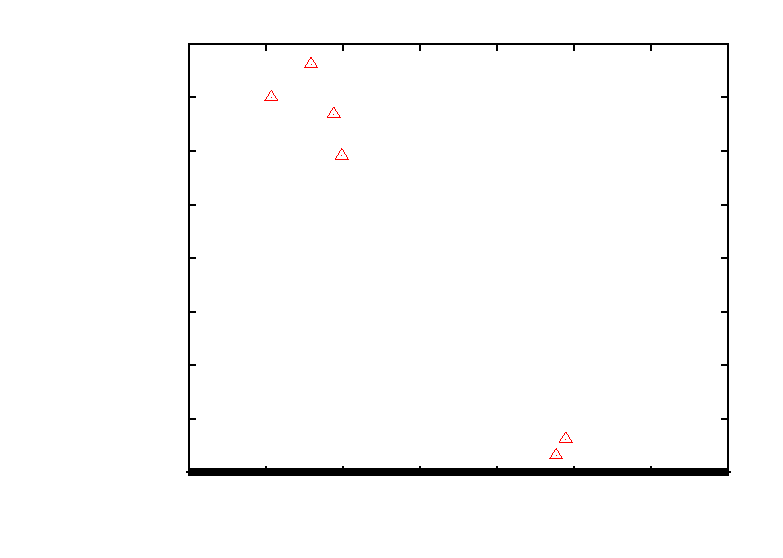
\includegraphics{fig/klight1}}%
    \gplfronttext
  \end{picture}%
\endgroup

%   \end{center}
% \end{figure}

% \begin{figure}
%   \begin{center}
%     % GNUPLOT: LaTeX picture with Postscript
\begingroup
  \makeatletter
  \providecommand\color[2][]{%
    \GenericError{(gnuplot) \space\space\space\@spaces}{%
      Package color not loaded in conjunction with
      terminal option `colourtext'%
    }{See the gnuplot documentation for explanation.%
    }{Either use 'blacktext' in gnuplot or load the package
      color.sty in LaTeX.}%
    \renewcommand\color[2][]{}%
  }%
  \providecommand\includegraphics[2][]{%
    \GenericError{(gnuplot) \space\space\space\@spaces}{%
      Package graphicx or graphics not loaded%
    }{See the gnuplot documentation for explanation.%
    }{The gnuplot epslatex terminal needs graphicx.sty or graphics.sty.}%
    \renewcommand\includegraphics[2][]{}%
  }%
  \providecommand\rotatebox[2]{#2}%
  \@ifundefined{ifGPcolor}{%
    \newif\ifGPcolor
    \GPcolorfalse
  }{}%
  \@ifundefined{ifGPblacktext}{%
    \newif\ifGPblacktext
    \GPblacktextfalse
  }{}%
  % define a \g@addto@macro without @ in the name:
  \let\gplgaddtomacro\g@addto@macro
  % define empty templates for all commands taking text:
  \gdef\gplbacktext{}%
  \gdef\gplfronttext{}%
  \makeatother
  \ifGPblacktext
    % no textcolor at all
    \def\colorrgb#1{}%
    \def\colorgray#1{}%
  \else
    % gray or color?
    \ifGPcolor
      \def\colorrgb#1{\color[rgb]{#1}}%
      \def\colorgray#1{\color[gray]{#1}}%
      \expandafter\def\csname LTw\endcsname{\color{white}}%
      \expandafter\def\csname LTb\endcsname{\color{black}}%
      \expandafter\def\csname LTa\endcsname{\color{black}}%
      \expandafter\def\csname LT0\endcsname{\color[rgb]{1,0,0}}%
      \expandafter\def\csname LT1\endcsname{\color[rgb]{0,1,0}}%
      \expandafter\def\csname LT2\endcsname{\color[rgb]{0,0,1}}%
      \expandafter\def\csname LT3\endcsname{\color[rgb]{1,0,1}}%
      \expandafter\def\csname LT4\endcsname{\color[rgb]{0,1,1}}%
      \expandafter\def\csname LT5\endcsname{\color[rgb]{1,1,0}}%
      \expandafter\def\csname LT6\endcsname{\color[rgb]{0,0,0}}%
      \expandafter\def\csname LT7\endcsname{\color[rgb]{1,0.3,0}}%
      \expandafter\def\csname LT8\endcsname{\color[rgb]{0.5,0.5,0.5}}%
    \else
      % gray
      \def\colorrgb#1{\color{black}}%
      \def\colorgray#1{\color[gray]{#1}}%
      \expandafter\def\csname LTw\endcsname{\color{white}}%
      \expandafter\def\csname LTb\endcsname{\color{black}}%
      \expandafter\def\csname LTa\endcsname{\color{black}}%
      \expandafter\def\csname LT0\endcsname{\color{black}}%
      \expandafter\def\csname LT1\endcsname{\color{black}}%
      \expandafter\def\csname LT2\endcsname{\color{black}}%
      \expandafter\def\csname LT3\endcsname{\color{black}}%
      \expandafter\def\csname LT4\endcsname{\color{black}}%
      \expandafter\def\csname LT5\endcsname{\color{black}}%
      \expandafter\def\csname LT6\endcsname{\color{black}}%
      \expandafter\def\csname LT7\endcsname{\color{black}}%
      \expandafter\def\csname LT8\endcsname{\color{black}}%
    \fi
  \fi
  \setlength{\unitlength}{0.0500bp}%
  \begin{picture}(7200.00,5040.00)%
    \gplgaddtomacro\gplbacktext{%
      \csname LTb\endcsname%
      \put(1254,660){\makebox(0,0)[r]{\strut{}$8.0$}}%
      \put(1254,1175){\makebox(0,0)[r]{\strut{}$9.0$}}%
      \put(1254,1689){\makebox(0,0)[r]{\strut{}$10.0$}}%
      \put(1254,2204){\makebox(0,0)[r]{\strut{}$11.0$}}%
      \put(1254,2718){\makebox(0,0)[r]{\strut{}$12.0$}}%
      \put(1254,3233){\makebox(0,0)[r]{\strut{}$13.0$}}%
      \put(1254,3747){\makebox(0,0)[r]{\strut{}$14.0$}}%
      \put(1254,4262){\makebox(0,0)[r]{\strut{}$15.0$}}%
      \put(1254,4776){\makebox(0,0)[r]{\strut{}$16.0$}}%
      \put(1386,440){\makebox(0,0){\strut{}$ 0$}}%
      \put(2163,440){\makebox(0,0){\strut{}$ 10$}}%
      \put(2940,440){\makebox(0,0){\strut{}$ 20$}}%
      \put(3717,440){\makebox(0,0){\strut{}$ 30$}}%
      \put(4495,440){\makebox(0,0){\strut{}$ 40$}}%
      \put(5272,440){\makebox(0,0){\strut{}$ 50$}}%
      \put(6049,440){\makebox(0,0){\strut{}$ 60$}}%
      \put(6826,440){\makebox(0,0){\strut{}$ 70$}}%
      \put(220,2718){\rotatebox{90}{\makebox(0,0){\strut{}Lat\^encia em $\mu s$}}}%
      \put(4106,110){\makebox(0,0){\strut{}Tempo de execu\c{c}\~ao em $s$}}%
    }%
    \gplgaddtomacro\gplfronttext{%
    }%
    \gplbacktext
    \put(0,0){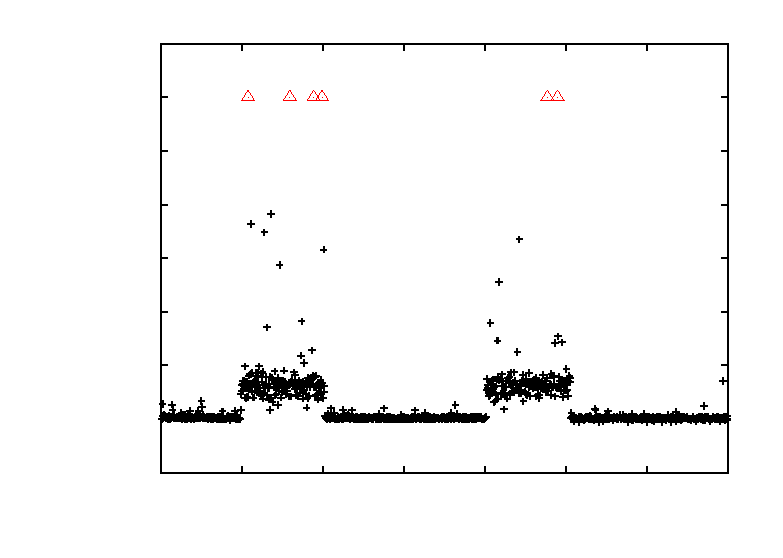
\includegraphics{fig/klight2}}%
    \gplfronttext
  \end{picture}%
\endgroup

%   \end{center}
% \end{figure}

% \begin{figure}
%   \begin{center}
%     \input{fig/klight3}
%   \end{center}
% \end{figure}

